\section{GraphRD7 Klassenreferenz}
\label{classGraphRD7}\index{GraphRD7@{GraphRD7}}
Klassendiagramm für GraphRD7::\begin{figure}[H]
\begin{center}
\leavevmode
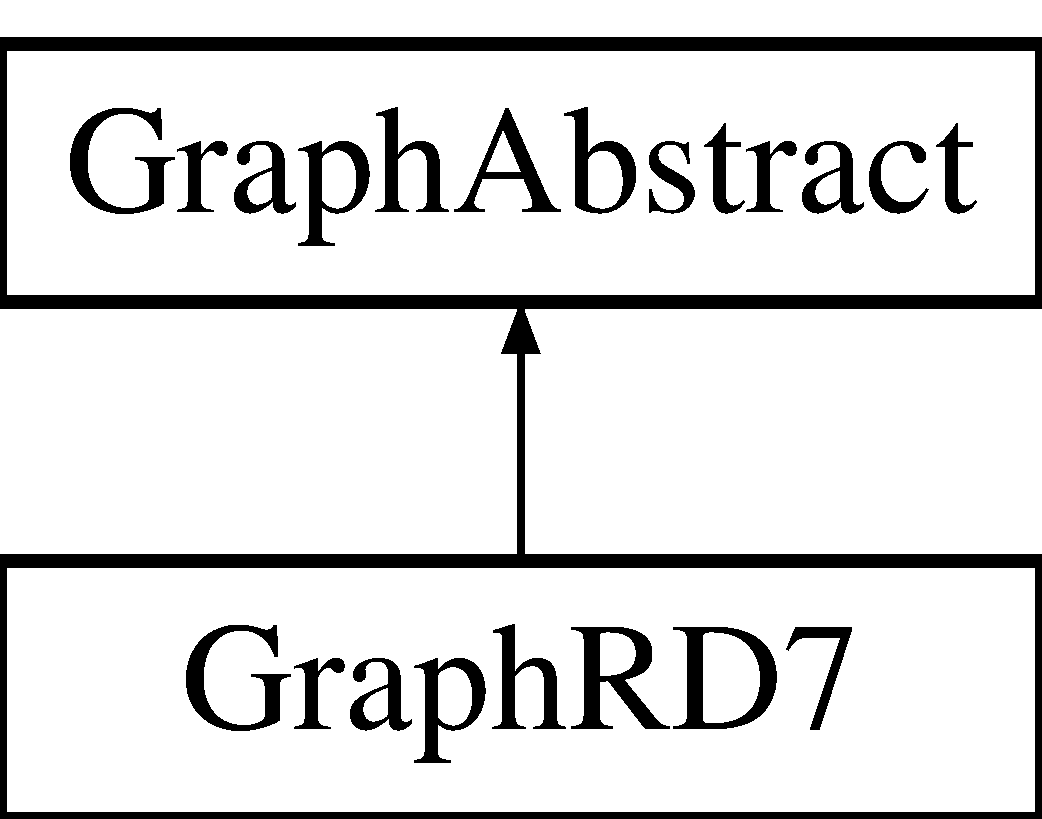
\includegraphics[height=2cm]{classGraphRD7}
\end{center}
\end{figure}
\subsection*{Öffentliche Methoden}
\begin{CompactItemize}
\item 
{\bf GraphRD7} (\$graphId)
\end{CompactItemize}


\subsection{Ausführliche Beschreibung}


Definiert in Zeile 7 der Datei class.GraphRD7.php.

\subsection{Dokumentation der Elementfunktionen}
\index{GraphRD7@{GraphRD7}!GraphRD7@{GraphRD7}}
\index{GraphRD7@{GraphRD7}!GraphRD7@{GraphRD7}}
\subsubsection{\setlength{\rightskip}{0pt plus 5cm}GraphRD7.GraphRD7 (\$ {\em graphId})}\label{classGraphRD7_42fd9702d8b35c73f7d9f75baf07452c}




Definiert in Zeile 9 der Datei class.GraphRD7.php.

Die Dokumentation für diese Klasse wurde erzeugt aufgrund der Datei:\begin{CompactItemize}
\item 
{\bf class.GraphRD7.php}\end{CompactItemize}
